% From the public sources to the files StormCrews ships. Compile with pdflatex; the paper includes the PDF and the
% README uses a PNG rendered from it, so both show the same drawing.
\documentclass[tikz,border=2pt]{standalone}
\usepackage[T1]{fontenc}
\usepackage{newtxtext,newtxmath}
\usetikzlibrary{arrows.meta,fit}
\begin{document}
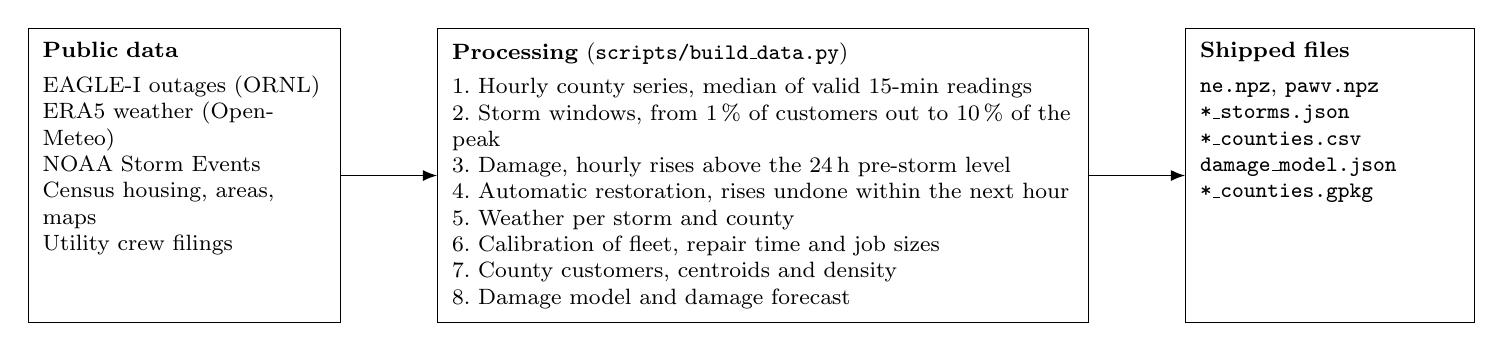
\begin{tikzpicture}[
  font=\footnotesize,
  txt/.style={inner sep=5pt, align=left, anchor=north west},
  box/.style={draw, line width=0.4pt, inner sep=0pt},
  arr/.style={-{Latex[length=1.8mm,width=1.4mm]}, line width=0.5pt}]

\node[txt, text width=3.6cm] (src) at (0,0) {%
  \textbf{Public data}\\[3pt]
  EAGLE-I outages (ORNL)\\
  ERA5 weather (Open-Meteo)\\
  NOAA Storm Events\\
  Census housing, areas, maps\\
  Utility crew filings};

\node[txt, text width=7.9cm] (proc) at (5.2,0) {%
  \textbf{Processing} (\texttt{scripts/build\_data.py})\\[3pt]
  1.\ Hourly county series, median of valid 15-min readings\\
  2.\ Storm windows, from 1\,\% of customers out to 10\,\% of the peak\\
  3.\ Damage, hourly rises above the 24\,h pre-storm level\\
  4.\ Automatic restoration, rises undone within the next hour\\
  5.\ Weather per storm and county\\
  6.\ Calibration of fleet, repair time and job sizes\\
  7.\ County customers, centroids and density\\
  8.\ Damage model and damage forecast};

\node[txt, text width=3.3cm] (out) at (14.7,0) {%
  \textbf{Shipped files}\\[3pt]
  \texttt{ne.npz}, \texttt{pawv.npz}\\
  \texttt{*\_storms.json}\\
  \texttt{*\_counties.csv}\\
  \texttt{damage\_model.json}\\
  \texttt{*\_counties.gpkg}};

% three frames of the same height, text at the top
\node[box, fit={(src.north west) (src.south east) (src.east |- proc.south)}] (bsrc) {};
\node[box, fit={(proc.north west) (proc.south east) (proc.east |- src.south)}] (bproc) {};
\node[box, fit={(out.north west) (out.east |- src.south) (out.east |- proc.south)}] (bout) {};

\draw[arr] (bsrc.east) -- (bproc.west);
\draw[arr] (bproc.east) -- (bout.west);
\end{tikzpicture}
\end{document}
